\documentclass[a4paper,journal]{IEEEtran}

\usepackage{graphicx}
\usepackage{amsmath,amssymb}
\usepackage{bm}
\usepackage{booktabs}
\usepackage{float}
\usepackage{adjustbox}
\usepackage{placeins}
\usepackage{balance} % equalise the two columns of the last page
\usepackage[colorlinks=true,linkcolor=blue,citecolor=blue,urlcolor=blue]{hyperref}

\newcommand{\vect}[1]{\mathbf{#1}}
\raggedbottom % no stretched gaps when a figure moves to the next column

\begin{document}

\title{Can a graph neural network replace a symplectic integrator for small-$N$ gravitational dynamics?}

\author{Abel Ephrem%
\thanks{Department of Physics, Imperial College London. Independent project, November 2026. Code and data: \url{https://github.com/abelephrem/nbody-integrator-study}.}}

\markboth{Abel Ephrem}{Abel Ephrem}

\maketitle

\begin{abstract}
We ask whether a graph neural network (GNN) can replace a symplectic integrator for small-$N$ gravitational dynamics (two to ten bodies). For the systems studied here it cannot. Comparing Euler, fourth-order Runge--Kutta (RK4) and Leapfrog on Kepler orbits, we find that long-time behaviour is governed by the \emph{structure} of a method's error rather than its size: RK4's energy error can be smaller than Leapfrog's, but it accumulates as a slow inward spiral, while Leapfrog's stays bounded. A GNN with central, equal-and-opposite pair messages inherits much of this structure: it learns the force to a median error of $0.6\%$, recovers the inverse-square law at short range, and conserves momentum and angular momentum to round-off. What it cannot remove is the size of its force error. In chaotic clusters it starts each trajectory further from the reference than a $10^{-6}$ perturbation does, so trajectories separate about twice as early. On two-body orbits the best model follows the orbit for a median of four periods, with a bounded energy error over 1000 times Leapfrog's (about 50 times in clusters). At an extrapolated mass ratio of 15, a model weighted towards quiet phases lasts one period, one weighted towards close encounters six. Each force evaluation is also 8--14 times slower than direct summation.
\end{abstract}


%=====================================================================
\section{Introduction}
%=====================================================================

\IEEEPARstart{T}{he} gravitational $N$-body problem has no general closed-form solution for $N\ge3$ and is studied by numerical integration \cite{Aarseth2003}. The choice of integrator is not decided by formal accuracy alone: symplectic methods such as Leapfrog preserve the geometric structure of Hamiltonian flow, which bounds their energy error over long times \cite{Hairer2006}, while higher-order methods such as RK4 are more accurate per step but carry no such guarantee. Machine-learned surrogates are a more recent alternative. Graph networks can simulate particle systems \cite{Battaglia2016,SanchezGonzalez2020} and recover force laws from $N$-body data \cite{Cranmer2020}; other models build in conservation laws \cite{Greydanus2019} or replace the integrator altogether \cite{Breen2020}. A learned model that is to stand in for a symplectic integrator should be judged by what makes that integrator worth using: not only the accuracy of each step, but how its errors behave over many.

We apply that standard to systems of two to ten bodies. Section~\ref{sec:theory} develops the expectations: why the long-time behaviour of an integrator is governed by the structure of its error (its symmetry, its direction, and whether it can accumulate) rather than its size, and how much of that structure a learned force can be given by construction. Section~\ref{sec:methods} describes the integration schemes, the dataset, the training and the comparison protocol. Section~\ref{sec:results} tests the expectations and then measures what the construction cannot supply: a force error of finite size, whose consequences for trajectories, conserved quantities and cost decide the title question. Section~\ref{sec:conclusion} concludes.

%=====================================================================
\section{Theory}\label{sec:theory}
%=====================================================================

\subsection{Equations of motion and units}\label{sec:eom}

Bodies interact through Newtonian gravity with Plummer softening $\varepsilon$,
\begin{equation}
\ddot{\vect r}_i=\sum_{j\neq i}\frac{G m_j(\vect r_j-\vect r_i)}{\left(|\vect r_j-\vect r_i|^2+\varepsilon^2\right)^{3/2}} ,
\label{eq:force}
\end{equation}
with every system nondimensionalised. Masses are measured in units of the system's total mass $M$, lengths in units of its virial radius $R=GM^2/2|E|$ (with $E$ the total energy), and times in units of
\begin{equation}
T=\sqrt{R^3/GM},
\end{equation}
so that $G=M=R=1$ and velocities are measured in units of $\sqrt{GM/R}$. In these units the equations of motion are the same for systems of any size or mass, so a learned force has to represent a single dimensionless law rather than one per system.

\subsection{Integrator error structure}\label{sec:thint}

We consider three explicit integrators at fixed step $h$: Euler (order 1), fourth-order Runge--Kutta (RK4, order 4) and kick--drift--kick Leapfrog (order 2). The order of a method bounds the error of one step; over many steps, what matters is whether those errors cancel or add. Three properties of an error decide this: its symmetry, its direction, and whether it can accumulate.

For fixed $h$, the Leapfrog trajectory is the exact flow of a modified Hamiltonian $\tilde H=H+h^2H_2+O(h^4)$, conserved up to terms that are exponentially small over our integration times \cite{Hairer2006}. The error in the true energy is then
\begin{equation}
H(t)-H(0)=-h^2\left[H_2(t)-H_2(0)\right]+O(h^4),
\label{eq:modham}
\end{equation}
a difference between two values of a function of the state. Such an error cannot accumulate, whatever its size: the growth exponent $q$ of its envelope in time should be zero. The same expression predicts how the maximum error scales with $h$ (exponent $s$): for a central force $H_2$ is constant on a circular orbit, so the $h^2$ term cancels and $s=4$, while on an eccentric orbit $s=2$ (Appendix~\ref{app:leapfrog}).

RK4 has no conserved modified energy. For a linear oscillator of angular frequency $\omega$, one RK4 step multiplies the squared amplitude by
\begin{equation}
|R(\theta)|^2=1-\frac{\theta^6}{72}+O(\theta^8),\qquad\theta=\omega h .
\end{equation}
The leading truncation error changes only the phase; the amplitude first changes at order $\theta^6$, and always as a loss. Losses of one sign add over $t/h$ steps, predicting $|\Delta E/E|\propto h^5t$: the energy error should scale as the fifth power of the step size ($s=5$) and grow linearly in time ($q=1$). The linear model fixes these exponents, not the prefactor of the nonlinear Kepler problem (Appendix~\ref{app:rk4}). The error is also directional: energy is only ever lost, and a Kepler orbit that loses energy while keeping its shape satisfies
\begin{equation}
|\Delta E/E_0|=2\,|\Delta L/L_0| ,
\label{eq:spiral}
\end{equation}
so an RK4 orbit should be a slow inward spiral.

Leapfrog, by contrast, should conserve angular momentum to round-off, and for a structural reason: each kick applies central, equal-and-opposite impulses to pairs of bodies and each drift moves bodies along their velocities, so neither can change the total angular momentum, whatever the step size. RK4 and Euler do not inherit this property of the exact dynamics. Euler, finally, is neither symplectic nor accurate; its error is free to grow until it is as large as the orbit.

\subsection{Building structure into a learned force}\label{sec:thgnn}

Leapfrog's guarantees follow from how its update is built, not from its accuracy. A learned force can be designed on the same principle: physical structure goes into the form of the model, and only the force law is left to be learned.

Each snapshot is a fully connected graph of bodies; gravity is long-range and $N\le10$, so no distance cutoff \cite{SanchezGonzalez2020} is used. The inputs are the masses and the displacements between bodies; velocity and absolute position are excluded because the acceleration depends on neither. After one round of message passing, a body's acceleration is the plain \emph{sum} of its incoming messages, so contributions superpose as forces do. Three message designs, D1, D2 and D3, add one assumption at a time (Table~\ref{tab:designs}): in D1 the message is an unconstrained vector; in D2 it points along the line joining the two bodies; in D3 it is, in addition, equal and opposite for each pair. None is told the inverse-square law or the mass dependence.

\begin{table}[H]
\caption{Message from body $j$ to body $i$. $\hat{\vect d}_{ij}$: unit vector from $i$ towards $j$. $s$: scalar output of a multilayer perceptron.}
\label{tab:designs}
\centering
\begin{adjustbox}{max width=\columnwidth}
\begin{tabular}{lll}
\toprule
 & Message & Built in\\
\midrule
D1 & free 3-vector & pairwise sum\\
D2 & $e^{s(m_j,\,r_{ij})}\,\hat{\vect d}_{ij}$ & central\\
D3 & $e^{s(m_im_j,\,m_i+m_j,\,r_{ij})}\,\hat{\vect d}_{ij}/m_i$ & central, Newton~3\\
\bottomrule
\end{tabular}
\end{adjustbox}
\end{table}

D3 enforces Newton's third law for any network weights: its scalar $s$ is symmetric in $i$ and $j$ while $\hat{\vect d}_{ij}$ changes sign, so
\begin{equation}
m_i\vect a_{i\leftarrow j}=-m_j\vect a_{j\leftarrow i} .
\label{eq:newton3}
\end{equation}
This has two consequences. First, every D3 force evaluation consists of central, equal-and-opposite pair forces, exactly the property that makes a Leapfrog kick conserve momentum and angular momentum (Sec.~\ref{sec:thint}); D3 inside Leapfrog therefore conserves both by construction. Second, each D3 pair force is central with a magnitude that, for given masses, depends only on separation. It is therefore minus the gradient of a learned pair potential, a function of separation alone. Summing these over all pairs gives a learned potential energy $U_L$, and the learned dynamics conserve the corresponding total energy
\begin{equation}
H_L=T+U_L ,
\label{eq:hl}
\end{equation}
where $T$ is the kinetic energy. D2 has no conserved energy in general: for unequal masses its pair forces are not equal and opposite, and its force field is not the gradient of any potential. In this model, building in the third law is also what makes the learned force conservative.

What a rollout is judged by, however, is the true energy $H=T+U$, with $U$ the potential energy of the softened force, Eq.~\eqref{eq:force}. The two energies differ only through their potentials, $H-H_L=U-U_L$, the mismatch between the true and learned potentials. If $H_L$ is conserved exactly, the measured energy error is the change of this mismatch between the current and initial configurations: like Leapfrog's error in Eq.~\eqref{eq:modham}, a difference of a function of the state, with a size set by the force error. On a periodic orbit, where the same configurations recur, this error should stay bounded. In a cluster, where a close encounter with a third body can leave a binary (a bound pair of bodies) permanently tighter, the mismatch settles at a new value and the error can step to a new level and stay there.

No property of this construction constrains the \emph{size} of the force error. That is left to training, and Sec.~\ref{sec:results} measures what it costs.

%=====================================================================
\section{Methods}\label{sec:methods}
%=====================================================================

\subsection{Integration}\label{sec:integration}

The fixed-step comparison of Sec.~\ref{sec:integrators} follows two unsoftened Kepler orbits, one circular and one eccentric ($e=0.5$), for 300 orbits at 400 steps per orbit, with step-size scans for the scaling exponents (Appendices \ref{app:leapfrog} and \ref{app:rk4}).

Close encounters in clusters are too fast for any affordable fixed step, so the dataset and all rollouts use Leapfrog with substeps recomputed at every substep from the largest acceleration,
\begin{equation}
h_k=\frac{1}{n_\mathrm{res}}\sqrt{\frac{\varepsilon}{a_{\max}(t_k)}},\qquad n_\mathrm{res}=96 .
\label{eq:substep}
\end{equation}
Because $h_k$ depends on the instantaneous state, this scheme is neither symplectic nor time-reversible, and the fixed-step bound on the energy error does not formally apply \cite{Hut1995}. We therefore report its energy behaviour empirically (Sec.~\ref{sec:energy}, Appendix~\ref{app:adaptive}).

\subsection{Dataset}\label{sec:data}

The dataset has 360 trajectories: 100 two-body orbits followed for 25.5 periods and 260 clusters of three to eight bodies followed for 20 time units, all with one softening, $\varepsilon=0.002$ in units of $R$, since a network can learn only one force law. Of these, 208 are used for training, 36 for validation and 36 for testing. A further 80 \emph{holdout} files each move one setting (eccentricity, mass ratio, $N$ up to 10, or virial ratio) to an interpolated or extrapolated value (Appendix~\ref{app:data}). Every stored acceleration satisfies Eq.~\eqref{eq:force} exactly, so the training targets do not depend on integration error; the integrator determines only which states are visited.

\subsection{Training}\label{sec:training}

Models are trained on the stored accelerations with a relative-error loss (Appendix~\ref{app:training}), weighted in one of two ways: \emph{time} weighting counts each snapshot by the time it represents, emphasising quiet phases, while \emph{kick} weighting counts each body by $|\vect a_i|\Delta t$, emphasising close encounters. The models rolled out are the kick- and time-weighted D3 (kick-D3, time-D3) and, on test files, D2.

\subsection{Rollout and comparison protocol}\label{sec:protocol}

Every rollout uses the adaptive Leapfrog of Sec.~\ref{sec:integration} with the substep always computed from the \emph{true} force at the run's current state. Only the force used in the kick differs, so differences from the reference are due to the learned force alone. Run with the true force, this loop reproduces all 115 stored test and holdout trajectories exactly.

For clusters we measure the root-mean-square distance $\delta(t)$ between corresponding bodies in a rollout and its reference, and define the \emph{horizon} as the first time $\delta\ge0.1$, or $10\%$ of the virial radius. Clusters are chaotic, so a rollout would separate from its reference even with an almost perfect force. To measure what chaos alone produces, each cluster is also run three times with the true force from positions displaced by $10^{-6}$.

To compare growth rates, we fit the slope of $\log\delta$ against $t$ between $\delta=10^{-4}$ and $0.1$ for every run. This is a finite-time, finite-size divergence rate, not a Lyapunov exponent: the window is short and growth is often step-like at encounters (many fits have $R^2<0.9$). We use it only to compare runs of the same cluster over the same range of $\delta$. A cluster is counted as showing a model contribution if the GNN's slope is at least 1.5 times the mean slope of its perturbed runs, a conventional threshold fixed before any model result. Treating each perturbed run as a pretend model against the other two gives the noise level of this count (Appendix~\ref{app:slopes}). All comparison rules were fixed before any model rollout was analysed.

Compute cost is measured per force evaluation on one CPU thread without batching.

%=====================================================================
\section{Results and discussion}\label{sec:results}
%=====================================================================

\subsection{Classical integrators}\label{sec:integrators}

Judged by formal accuracy, the integrators behave as expected: the measured convergence orders are 0.90, 4.37 and 2.00 for Euler, RK4 and Leapfrog (Table~\ref{tab:integrators}), and RK4 is clearly the best. Over long runs the ranking changes, as Sec.~\ref{sec:thint} predicts. Euler's energy error reaches order unity within a few orbits. RK4's is small but grows linearly in time and scales as the fifth power of the step ($q=1.00$ and $0.90$, $s=5.0$ on both orbits), the signature of its accumulating amplitude loss, once a run is long enough for that term to dominate (Fig.~\ref{fig:integrators}, Appendix~\ref{app:rk4}). Leapfrog's error oscillates without growing ($q\le0.02$; Fig.~\ref{fig:leapfrog}) and scales as $h^4$ on the circular orbit and $h^2$ on the eccentric one (Appendix~\ref{app:leapfrog}). Size does not decide this: on the eccentric orbit, at the same step size, RK4's energy error after 300 orbits is still about 75 times \emph{smaller} than Leapfrog's.

\begin{table}[H]
\caption{Fixed-step integrators on Kepler orbits (300 orbits, 400 steps per orbit). $p$: convergence order (theory in brackets). $q$: growth exponent in time of the energy-error envelope. $s$: scaling exponent of the maximum energy error with $h$. Pairs are circular / eccentric.}
\label{tab:integrators}
\centering
\begin{adjustbox}{max width=\columnwidth}
\begin{tabular}{lccc}
\toprule
 & Euler & RK4 & Leapfrog\\
\midrule
$p$ & 0.90 (1) & 4.37 (4) & 2.00 (2)\\
$|\Delta E/E_0|_{\max}$, circ. & 0.82 & $5.0{\times}10^{-8}$ & $1.5{\times}10^{-8}$\\
$|\Delta E/E_0|_{\max}$, ecc. & 1.0 & $8.8{\times}10^{-6}$ & $6.7{\times}10^{-4}$\\
$q$ & saturates & 1.00 / 0.90 & 0.02 / 0.00\\
$s$ & -- & 5.0 / 5.0 & 4.0 / 2.0\\
$|\Delta L/L_0|_{\max}$, circ. & 1.4 & $2.5{\times}10^{-8}$ & $2.5{\times}10^{-14}$\\
$|\Delta L/L_0|_{\max}$, ecc. & 0.58 & $1.3{\times}10^{-6}$ & $6.0{\times}10^{-14}$\\
\bottomrule
\end{tabular}
\end{adjustbox}
\end{table}

\begin{figure}[H]
\centering
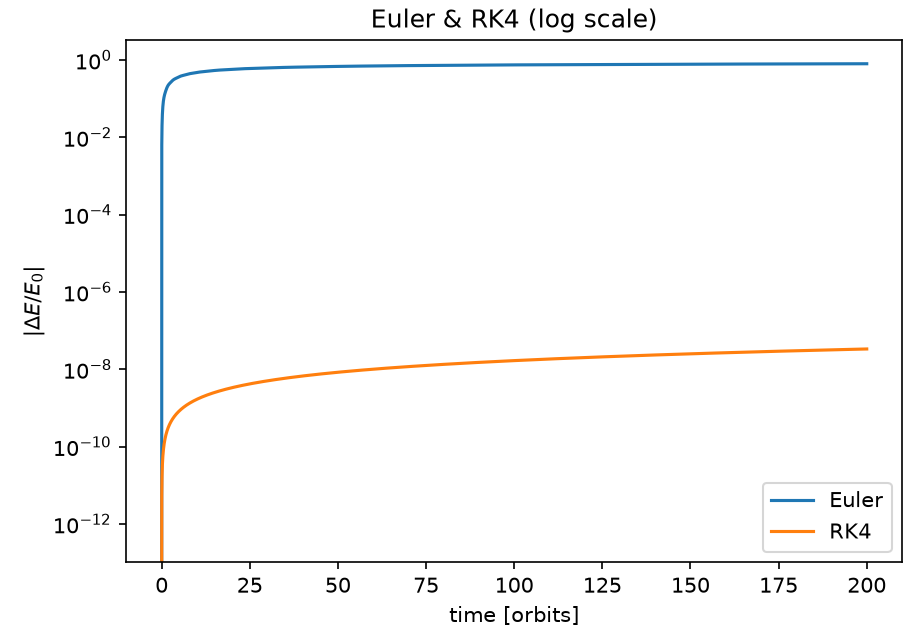
\includegraphics[width=\columnwidth]{figs/energy_drift_euler_rk4.png}
\caption{Energy error of Euler and RK4 on the circular Kepler orbit over 200 orbits at 400 steps per orbit, on a logarithmic scale. Euler's error saturates at order unity and RK4's grows steadily.}
\label{fig:integrators}
\end{figure}

\begin{figure}[H]
\centering
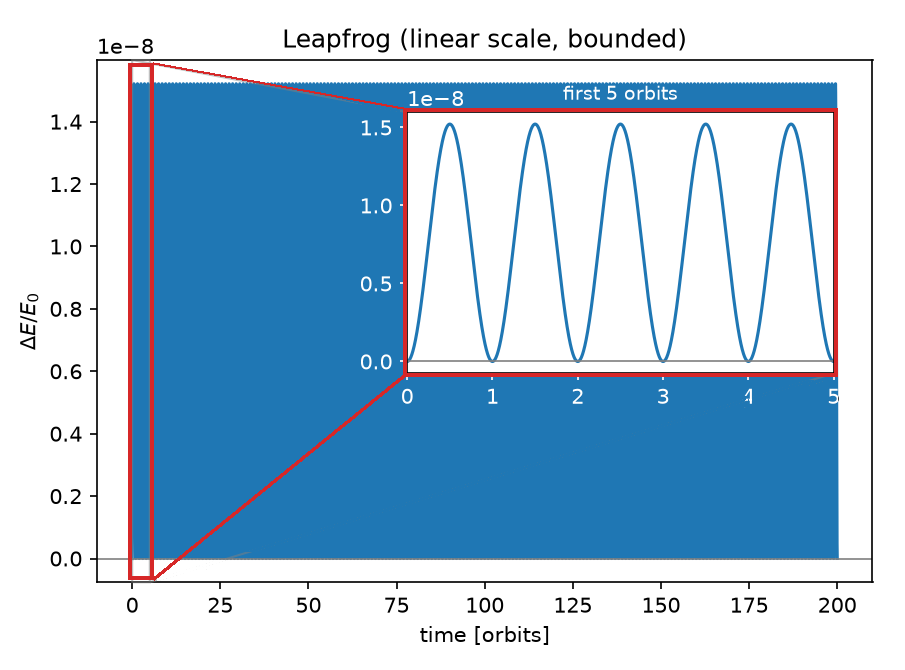
\includegraphics[width=\columnwidth]{figs/energy_drift_leapfrog.png}
\caption{Energy error of Leapfrog on the same orbit and step size as Fig.~\ref{fig:integrators}, on a linear scale. The inset (red frame) enlarges the first five orbits, marked by the red box. The error oscillates within a fixed band.}
\label{fig:leapfrog}
\end{figure}

The direction of the errors also follows Sec.~\ref{sec:thint}. RK4's energy and angular-momentum errors never change sign, and on the circular orbit they satisfy the spiral relation of Eq.~\eqref{eq:spiral} ($5.01\times10^{-8}$ and $2.50\times10^{-8}$): the RK4 orbit is a slow inward spiral. Leapfrog conserves angular momentum to round-off ($6\times10^{-14}$ or better), as its kick structure requires.

These results fix the reference. An RK4-generated dataset would consist of orbits that all contract, a bias a model could learn, and a reference whose own error grows would contaminate any long comparison. Leapfrog's error has no preferred direction and, at fixed step, does not grow. We select it for the character of its error, not its size.

\subsection{Learned force}\label{sec:learned}

Structure is necessary before it is helpful. The unconstrained D1 does not learn the force (median relative error $0.997$, no better than predicting zero), because a three-number output cannot represent magnitudes spread over eight decades. Writing the message as a strength $e^{s}$ along the line joining the bodies (D2) removes the difficulty: the median error falls to $0.59\%$, and the error stays well below that of predicting zero across the whole trained range (Fig.~\ref{fig:g1}). Adding Newton's third law (D3) costs no accuracy (median error $0.62\%$). The network also learns the law it was not given: the fitted exponent of the learned pair messages against separation is within $0.006$ of $-2$ between ten softening lengths and $r=1$; at larger separations, where pulls are weak, the kick-weighted models are less well constrained (Appendix~\ref{app:training}).

\begin{figure}[H]
\centering
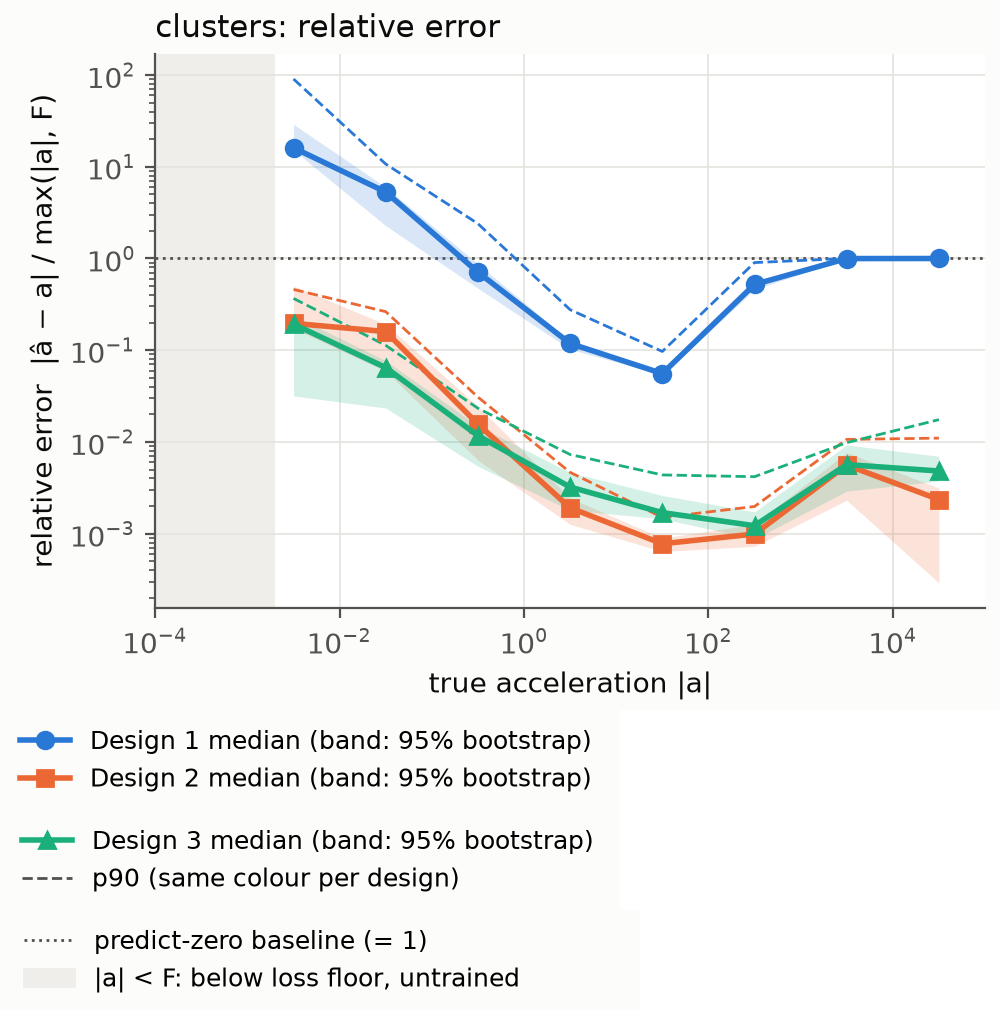
\includegraphics[width=0.75\columnwidth]{figs/per_decade_clusters.png}
\caption{One-step relative error of the kick-weighted models on the test clusters, by decade of the true acceleration. Lines are medians. Shaded bands show the uncertainty in each median: the range covering $95\%$ of the medians obtained when the 36 test files are resampled with replacement 1000 times (whole files are resampled because snapshots from one trajectory are correlated); dashed lines are 90th percentiles. Design 1 is D1, Design 2 is D2 and Design 3 is kick-D3. Grey region: below the loss floor $F$. Dotted line: the error of predicting zero.}
\label{fig:g1}
\end{figure}

The conservation designed into D3 (Sec.~\ref{sec:thgnn}) holds at machine precision in practice. On single snapshots its momentum residual is $3.2\times10^{-8}$, the single-precision floor of the true accelerations ($2.3\times10^{-8}$), against $3.0\times10^{-4}$ for D2. D3 thus has the symmetries that separated Leapfrog from RK4. What it does not have is the exact force.

\subsection{Trajectory divergence}\label{sec:divergence}

A force error of $0.6\%$ is far larger than any integration error in this study, and the constraints of Sec.~\ref{sec:thgnn} do not reduce it. Its first consequence is how long a rollout tracks the reference. The GNN rollouts separate sooner than the perturbed runs of Sec.~\ref{sec:protocol}: on test clusters the median horizon is 1.6 to 1.7 time units against 3.4 to 4.0, and cluster by cluster it is shorter by a median factor of 1.8 to 2.4 across models and splits. Either the learned force makes the separation grow faster than chaos does, or it produces a larger separation at the outset, which chaos then amplifies at its usual rate. The curves suggest the second: a GNN rollout passes $\delta=10^{-4}$ at $t\approx0.1$, a perturbed run at $t\approx1.7$ (Fig.~\ref{fig:g2}).

\begin{figure}[H]
\centering
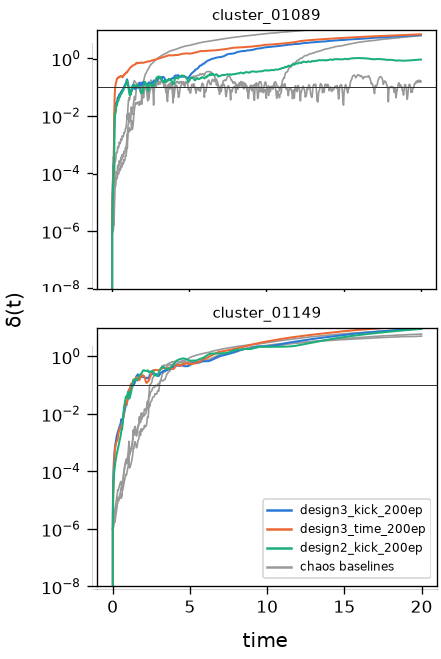
\includegraphics[width=\columnwidth]{figs/divergence_two_clusters.png}
\caption{Divergence $\delta(t)$ from the reference for the two test clusters whose kick-D3 slope ratios lie on either side of the median of the 18 voting clusters (1.31 and 1.36; median 1.33). Blue: kick-D3 (\texttt{design3\_kick\_200ep}); orange: time-D3; green: D2; grey: three true-force runs started from positions displaced by $10^{-6}$. Horizontal line: the horizon threshold $\delta=0.1$. Time is in $N$-body units. Panels are taken from the full set of 20 test clusters in the repository.}
\label{fig:g2}
\end{figure}

The slope comparison distinguishes the two. Kick-D3 and time-D3 are each counted in 7 of 18 test clusters, and in 12 and 17 of 58 holdout clusters, against a noise level of at most 2 of 18 and 4 of 58 from the pretend models; D2, at 3 of 18, is at the noise level, and RK4 with the true force, as a control, gives 0 and 5. The median slope ratio is between 1.03 and 1.33. The learned force therefore accelerates error growth in a minority of clusters, by more than noise explains. In the majority, growth is consistent with the cluster's own divergence rate, and the shorter horizon is mainly the result of the larger initial error. The counts do not rank the models, since the ratios are correlated across models and the noise estimate is rough (Appendix~\ref{app:slopes}). Nor is there a penalty on holdout clusters once their stronger chaos is taken into account (Appendix~\ref{app:data}).

\subsection{Energy and angular momentum}\label{sec:energy}

The conservation properties built into D3 survive every rollout. D3 holds the angular momentum to $10^{-6}$--$10^{-5}$ of its scale over a cluster run, the level of single-precision round-off, while D2 loses $12\%$ (Fig.~\ref{fig:g3}). This does not make trajectories more accurate (D2's cluster horizons are no shorter than D3's): structure governs which quantities are conserved, not how closely a trajectory is followed.

\begin{figure}[H]
\centering
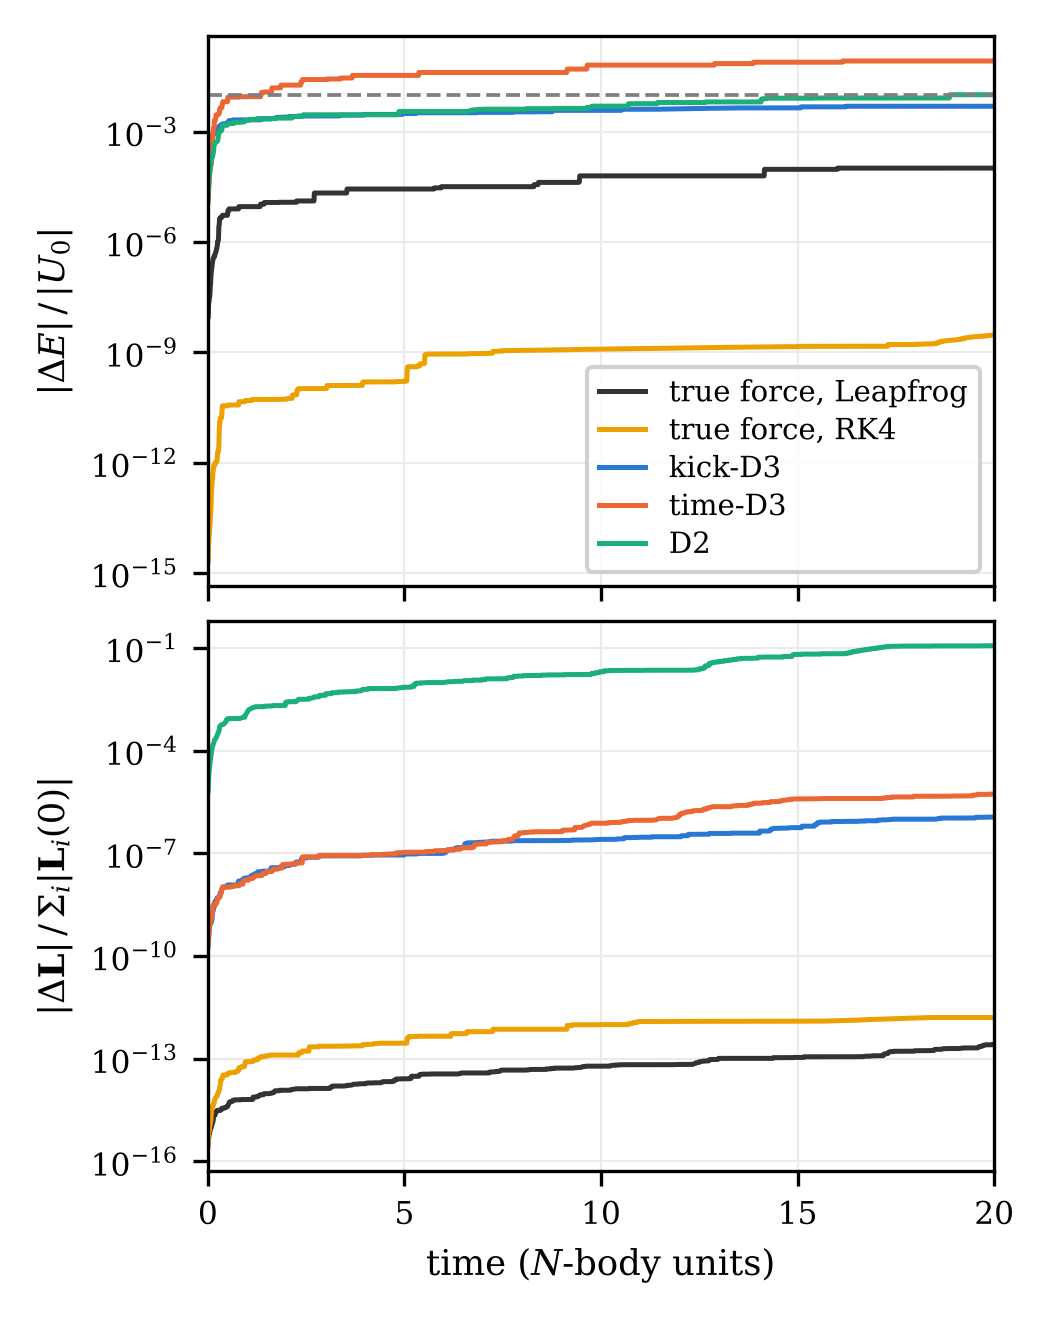
\includegraphics[width=\columnwidth]{figs/g3_clusters.png}
\caption{Conservation errors in the test-cluster rollouts. Top: energy error, relative to the initial potential energy $|U_0|$. Bottom: total angular-momentum error, relative to the sum of the bodies' initial angular-momentum magnitudes. Each curve is the largest error a run has reached by time $t$, taken as the median over the 20 test clusters. The true-force runs are Leapfrog (the reference) and RK4. Dashed line: the tolerance used to accept the dataset, shown for context only.}
\label{fig:g3}
\end{figure}

The energy behaves as the potential-mismatch picture of Sec.~\ref{sec:thgnn} anticipates. On two-body orbits, where the same configurations recur every period, every GNN's energy error is bounded with no trend, at $3.8\times10^{-4}$ of the initial potential energy $|U_0|$ for kick-D3 and $4.5\times10^{-4}$ for time-D3. The reference, through the same integrator, has an error of $2.5\times10^{-7}$, so this level is an offset due to the learned force. In clusters, configurations change irreversibly and the error steps at encounters. Kick-D3 remains mostly bounded (median maximum $4.9\times10^{-3}$; 6 of 20 test runs reach $1\%$), whereas time-D3's error rises in steps and reaches $1\%$ in 19 of 20, the behaviour expected of a force that is least accurate at close range, as time-D3's is (Sec.~\ref{sec:where}). We did not evaluate $H_L$, however, so a contribution from the adaptive step cannot be excluded.

The same caution applies to the reference, whose cluster energy error also rises in small steps at encounters, to a median maximum of $1.0\times10^{-4}$. Our measures cannot distinguish a slow drift of the adaptive scheme from the deepest encounter occurring late in a run. Either way, the reference error is about 50 times below that of the best GNN in clusters, and more than 1000 times below it on two-body orbits.

\subsection{Effect of loss weighting}\label{sec:where}

If the size of the force error limits a rollout, its distribution should decide which systems are followed well. The two weightings of Sec.~\ref{sec:training} test this, because they distribute a similar overall error in opposite ways (Table~\ref{tab:weighting}). In clusters, time-D3 is 2 to 70 times more accurate than kick-D3 at accelerations below about 100, and has the lower overall median ($0.23\%$); kick-D3 is 2 to 30 times more accurate above, where time-D3's error reaches about $6\%$ in the regime of close encounters. The summary number favours time weighting. The rollouts do not.

The cluster energy errors above are the first sign. Two-body orbits, which are not chaotic and so show model error undisguised, give a cleaner comparison (Table~\ref{tab:twobody}). On the 16 test orbits the weightings are level: kick-D3 has the longer horizon on nine and time-D3 on six, each on the orbits whose accelerations it fits better (Appendix~\ref{app:twobody}). Outside the training range they separate. On the two extrapolated holdout orbits kick-D3 keeps a horizon comparable to its test values (0.9 periods at $e=0.9$; 6.0 at mass ratio 15), while time-D3 falls to 0.2 and 1.0, having lasted 11.0 periods at the trained mass ratio 10. A one-step evaluation, with its reading rule fixed beforehand, finds time-D3's force error at mass ratio 15 to be four to five times its error at mass ratio 10, while kick-D3's does not rise. The collapse is thus consistent with an extrapolation failure of the force itself. With four distinct holdout orbits, this is an indication rather than a statistic.

Kick weighting is therefore the better choice for rollouts despite its higher median one-step error: what matters is whether the error is small where the dynamics are most sensitive to it.

\subsection{Computational cost}\label{sec:cost}

A surrogate less faithful than the method it replaces can still be worth using if it is cheaper. Here it is not. Under the timing conditions of Sec.~\ref{sec:protocol}, the true force takes 16 to 27\,$\mu$s per evaluation for $N=2$ to 10 and the GNN 180 to 280\,$\mu$s, a factor of 8 to 14. The graph is fully connected, so the GNN scales as $N^2$ like direct summation, with a larger constant.

\subsection{Discussion}\label{sec:answer}

For two to ten bodies, then, the answer to the title question is no (Table~\ref{tab:unified}). The classical and learned halves of the study reach this from opposite directions. Among integrators, the method with the larger error but the right structure is preferable over long times. For the learned force, the structure can be supplied by construction and is then preserved exactly, but it is not sufficient: the remaining error sets how far a trajectory starts from the truth and how far its energy sits from the true value, and its distribution decides which systems fail. A surrogate pays off when the true force is expensive or the model permits larger steps \cite{SanchezGonzalez2020,Cranmer2020,Breen2020}; neither holds for a closed-form sum over ten bodies under a fixed step rule.

\begin{table}[H]
\caption{Summary of the rollout comparison (test-set medians). Cluster horizons in $N$-body time units (Leapfrog: true-force runs perturbed by $10^{-6}$); time per force call at $N=10$.}
\label{tab:unified}
\centering
\footnotesize
\setlength{\tabcolsep}{3.5pt}
\begin{tabular}{lcccc}
\toprule
Method & Cluster $|\Delta E|/|U_0|$ & $|\Delta\vect L|$ (rel.) & Horizon & $\mu$s/call\\
\midrule
Leapfrog & $1.0{\times}10^{-4}$ & $3{\times}10^{-13}$ & 3.4--4.0 & 22\\
RK4 & $3.0{\times}10^{-9}$ & $2{\times}10^{-12}$ & 4.4 & 22$^{\ast}$\\
kick-D3 & $4.9{\times}10^{-3}$ & $1{\times}10^{-6}$ & 1.6 & 273\\
time-D3 & $8.4{\times}10^{-2}$ & $6{\times}10^{-6}$ & 1.7 & 280\\
D2 & $1.0{\times}10^{-2}$ & $0.12$ & 2.2 & 255\\
\bottomrule
\multicolumn{5}{l}{\scriptsize $^{\ast}$RK4 needs four force calls per step.}
\end{tabular}
\end{table}

The main limitations are a single training seed per rollout, small samples (18 and 58 clusters; 16 and 4 distinct two-body orbits), a rough noise estimate for the slope comparison, and timing on one unbatched CPU thread, which could change the constant but not the scaling. Evaluating $H_L$ along rollouts and using a time-symmetric step \cite{Hut1995} would remove the two main caveats.

%=====================================================================
\section{Conclusion}\label{sec:conclusion}
%=====================================================================

We asked whether a graph neural network can replace a symplectic integrator for systems of two to ten bodies. For the systems studied here it cannot.

The classical integrators set the standard. RK4 is the most accurate per step (measured order 4.37), yet its energy error grows linearly in time and always in the same direction, so its orbits spiral slowly inward. Leapfrog's energy error can be larger, as on the eccentric orbit, but it is bounded, because it is the change in a conserved modified energy, and its kicks conserve angular momentum to round-off. Over long times the structure of an error matters more than its size, which is why Leapfrog generates the reference.

Much of that structure can be built into a learned force. With central, equal-and-opposite pair messages (D3), the network learns gravity to a median one-step error of $0.6\%$, recovers the inverse-square law at short range without being told it, conserves momentum and angular momentum to single-precision round-off, and conserves a learned energy $H_L$ by construction. Without the central form (D1) it does not learn the force at all.

What cannot be built in is the size of the force error, and that error decides the outcome. In clusters it starts each trajectory further from the reference than a $10^{-6}$ perturbation does, so horizons are shorter by a median factor of 1.8 to 2.4; in most clusters the separation then grows at the cluster's own chaotic rate. It also offsets the measured energy, which stays bounded on two-body orbits but sits over 1000 times above Leapfrog's error, and about 50 times above it in clusters. Where the error lies matters as much as its average: weighting training towards close encounters gives a higher median one-step error but longer-lived rollouts, and at an extrapolated mass ratio of 15 a model weighted towards quiet phases lasts one period against six. With each evaluation 8 to 14 times slower than direct summation, the surrogate offers no speed to compensate.

A learned force may still pay off where the true force is expensive to evaluate or where the model allows larger steps. For our energy results, evaluating $H_L$ along rollouts and using a time-symmetric step are the natural next tests.

\vspace{2ex}
\noindent\rule{\columnwidth}{0.8pt}\par
\vspace{0.6ex}
{\centering\large\textsc{Appendices}\par}
\vspace{0.3ex}
\noindent\rule{\columnwidth}{0.8pt}\par
\vspace{1ex}
\appendices
%=====================================================================

\section{Leapfrog energy scaling}\label{app:leapfrog}

This appendix expands the scaling argument of Sec.~\ref{sec:thint} for Leapfrog. For a Hamiltonian $H=T+V$, the first correction $H_2$ in the modified Hamiltonian of Leapfrog is a fixed linear combination of $|\nabla V|^2$ and $\vect v^{\mathsf T}(\nabla\nabla V)\vect v$, with coefficients determined by the ordering of the kick and drift substeps \cite{Hairer2006}. For a central potential both quantities depend only on the separation $r$, the radial speed and the tangential speed, so $H_2$ takes a single value on a circular orbit, and since a time-symmetric method admits only even powers of $h$ the next term is of order $h^4$. The numerical trajectory starts from the exact circular initial conditions but follows the flow of $\tilde H$, for which those conditions are in general not circular; the departure is of order $h^2$, so along the numerical trajectory $H_2$ varies by an amount of order $h^2$. Multiplied by its prefactor $h^2$ and combined with the next term $h^4H_4$, this gives an energy error of order $h^4$. The measured maximum energy error falls by a factor of 16.0 for each halving of $h$ on the circular orbit and by 4.0 on the eccentric orbit (Fig.~\ref{fig:scaling}).

\begin{figure}[t]
\centering
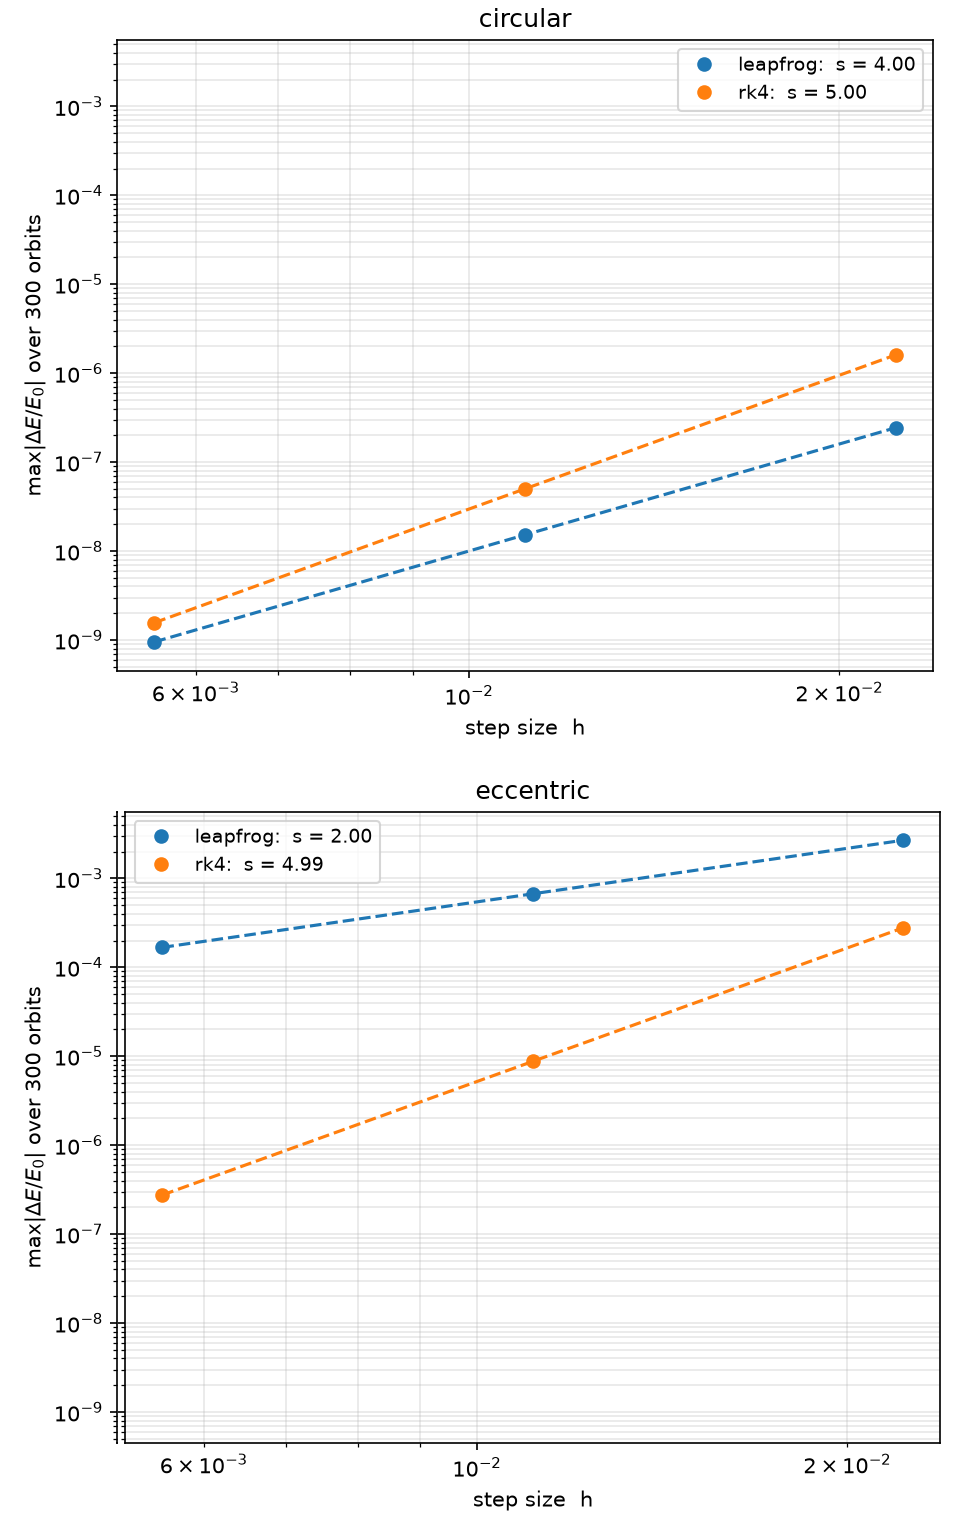
\includegraphics[width=0.85\columnwidth]{figs/long_runs_scaling.png}
\caption{Maximum energy error over 300 orbits against step size, for the circular (top) and eccentric (bottom) orbits, with the fitted exponents $s$ for Leapfrog and RK4.}
\label{fig:scaling}
\end{figure}

\section{RK4 energy error}\label{app:rk4}

This appendix expands the RK4 argument of Sec.~\ref{sec:thint} and tests it against the measured errors. A circular orbit of angular frequency $\omega$ can be written as a complex number obeying $\dot z=i\omega z$. One RK4 step multiplies $z$ by the Taylor series of $e^{i\theta}$, $\theta=\omega h$, truncated after the fourth power,
\begin{equation}
R(\theta)=1-\frac{\theta^2}{2}+\frac{\theta^4}{24}+i\left(\theta-\frac{\theta^3}{6}\right),
\end{equation}
whose squared modulus is
\begin{equation}
|R|^2=1-\frac{\theta^6}{72}+\frac{\theta^8}{576}.
\end{equation}
The leading error, $R-e^{i\theta}\approx-i\theta^5/120$, is perpendicular to $z$ to leading order and so changes its phase and not its length. Accumulated over $t/h$ steps, the loss in $|z|^2$ is
\begin{equation}
\frac{t}{h}\,\frac{\theta^6}{72}=\frac{\omega^6h^5t}{72}.
\end{equation}
The measured energy error falls by factors of 31.9 and 32.1 for each halving of $h$ on the circular orbit, and by 31.9 and 31.7 on the eccentric orbit, against $2^5=32$. (In the convergence fits of Table~\ref{tab:integrators}, the smallest RK4 steps reach round-off and are excluded, and Euler's fit uses only its smallest steps, since at larger ones its error is as large as the orbit.)

Over a short run the scaling is different. For five orbits of the eccentric case, the local slope of $\log\max|\Delta E/E_0|$ against $\log h$ rises smoothly from 4.2 at $h=10^{-3}$ to 5.0 at $h=0.046$ (Fig.~\ref{fig:setd}). This is described by two terms,
\begin{equation}
\max|\Delta E/E_0|\approx Ah^4+Bh^5t,
\end{equation}
the first representing an excursion of the energy at each periapsis passage that is largely reversed afterwards, and the second the accumulating loss. A fit of $A$ and $B$ to the five-orbit runs has a root-mean-square residual of $0.001$ in the natural logarithm ($A=4.60$, $B=772$ in the units of Sec.~\ref{sec:eom}). With $A$ and $B$ held fixed, the expression predicts the maximum errors of the independent 300-orbit runs to within $10\%$; there the second term supplies more than $98\%$ of the total, which is why those runs show $s=5$. That the first term does not grow with time is an assumption of this description that we have not tested separately.

\begin{figure}[H]
\centering
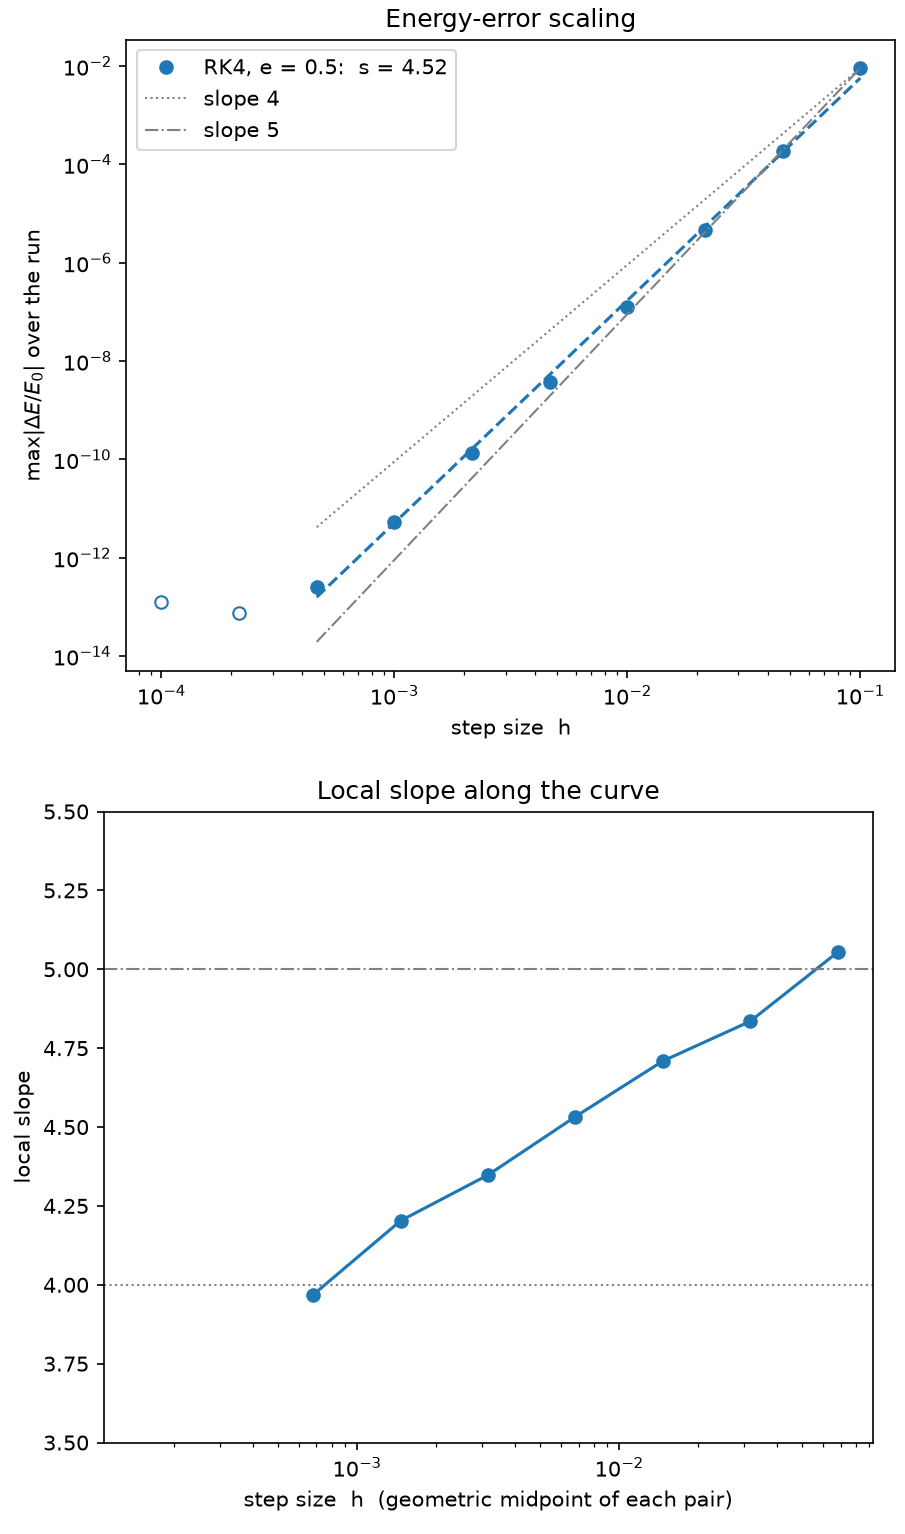
\includegraphics[width=0.85\columnwidth]{figs/energy_scaling.png}
\caption{RK4 on the eccentric ($e=0.5$) orbit over five orbits. Top: maximum energy error against step size, with a single power-law fit ($s=4.52$) and reference slopes of 4 and 5; open circles lie on the round-off floor and are excluded. Bottom: local slope between adjacent step sizes, which rises from about 4 to 5.}
\label{fig:setd}
\end{figure}

\section{Adaptive Leapfrog}\label{app:adaptive}

Two checks bear on the adaptive scheme of Eq.~\eqref{eq:substep}. First, one cluster with a large energy error was rerun at two substep resolutions and, for comparison, at two fixed step sizes. The coarser adaptive run drifted in energy, while the finer one was flat over the 20 time units of the run, and halving the step reduced the error fourfold for the adaptive and the fixed pair alike. Three flagged clusters were rerun at higher resolution and all flattened, but in only one did the system follow the same sequence of encounters, so only that one is a like-for-like comparison. We take this as evidence that the large errors seen at coarse resolution were due to under-resolved encounters. It is not a demonstration that the adaptive scheme conserves energy in general.

Second, the scheme imposes an upper limit on the step during close encounters and shortens the last substep to land on each stored time. The limit was active in 9 of the 20 test and 12 of the 59 holdout reference clusters, on $0.17\%$ and $0.06\%$ of all substeps, and on at most $4.3\%$ of the substeps of a single run. Runs in which it was active did not have larger energy errors (median maximum $4.4\times10^{-5}$ of $|U_0|$, against $1.0$ to $1.6\times10^{-4}$ for the others), though the two groups differ in their encounters and the comparison is not controlled. Because the step is always computed from the true force, the limit acts identically in reference and GNN runs.

\section{Dataset}\label{app:data}

Two-body orbits have eccentricity $e\in\{0,0.2,0.4,0.8\}$ and mass ratio in $\{1,3,7,10\}$. Clusters have $N\in\{3,4,5,7,8\}$, one heavier body of mass ratio in $\{1,3,7,10\}$, and initial virial ratio $Q\in[0.3,0.7]\cup[1.1,1.5]$. Files are split by whole trajectory. Each holdout file moves one setting to an interpolated or extrapolated value with the others at a trained baseline: $e=0.6$ or $0.9$; mass ratio 5 or 15; $N=6$ or 10; $Q$ in $(0.7,1.1)$ or $(1.6,1.8)$. Snapshots are stored more densely near periapsis and during close encounters. Three cluster runs exceed the energy tolerance used to accept the dataset ($|\Delta E|/|U_0|=10^{-2}$); they are kept for training, since their accelerations are exact, but are never used as references.

The holdout clusters are more chaotic than the test clusters (perturbed-run horizons of 2.8 to 3.2 against 3.4 to 4.0), so GNN horizons are shorter in absolute terms. Relative to each cluster's own perturbed runs the models do no worse than on the test set: the share of clusters showing a model contribution is $21\%$ (kick-D3) and $29\%$ (time-D3), against $39\%$ on test, and slope ratios and energy errors are at the test level. The nine holdout clusters whose closest approach falls below $0.2\varepsilon$, where training data are sparse, do no worse than the rest, although nine clusters can exclude only a large penalty.

\section{Training details}\label{app:training}

The loss is a weighted relative error with a floor $F=2\times10^{-3}$ on the denominator,
\begin{equation}
\mathcal L=\frac{\sum_i w_i\,|\hat{\vect a}_i-\vect a_i|^2/\max(|\vect a_i|,F)^2}{\sum_i w_i},
\end{equation}
where the sum runs over bodies and snapshots. Bodies with $|\vect a|<F$ make up $7\%$ of the data but carry a negligible share of the kick weight, so the lowest accelerations are effectively untrained under kick weighting. The multilayer perceptron has two hidden layers of 128 units with SiLU activations \cite{Elfwing2018}; masses and distances enter as logarithms, standardised with statistics of the training set. Training uses Adam \cite{Kingma2015} with a learning rate decaying exponentially from $10^{-3}$ to $10^{-4}$, batches of 512 graphs, and gradient-norm clipping \cite{Pascanu2013} at ten times the median norm of the preceding 100 steps, without which training of D3 collapsed. Models were trained for 200 epochs, after a test fixed in advance showed that doubling from 100 epochs improved D3 clearly in six of ten decades of $|\vect a|$. The weights at the final epoch are used throughout. Table~\ref{tab:onestep} lists the one-step results.

\begin{table}[H]
\caption{One-step results on the test set (seed 0; errors are medians). The momentum residual is $|\sum_im_i\hat{\vect a}_i|/\sum_im_i|\hat{\vect a}_i|$. $\beta$ is the fitted exponent of the pair-message magnitude against separation; the true force gives $-2.000$ in both ranges.}
\label{tab:onestep}
\centering
\begin{adjustbox}{max width=\columnwidth}
\begin{tabular}{lcccc}
\toprule
 & D1 & D2 & kick-D3 & time-D3\\
\midrule
relative error & 0.997 & 0.0059 & 0.0062 & 0.0023\\
direction error & $29^\circ$ & $0.018^\circ$ & $0.024^\circ$ & --\\
momentum residual & 0.75 & $3.0{\times}10^{-4}$ & $3.2{\times}10^{-8}$ & --\\
$\beta$, $0.1<r<1$ & -- & $-2.006$ & $-1.997$ & $-1.999$\\
$\beta$, $10<r<100$ & -- & $-3.13$ & $-1.40$ & $-1.98$\\
\bottomrule
\end{tabular}
\end{adjustbox}
\end{table}

Across three training seeds the median relative error is 0.56 to 0.59\% for D2 and 0.58 to 0.95\% for kick-D3. The momentum residual of D3 is at the single-precision floor for every seed. D2's momentum residual varies twentyfold between seeds. The time-weighted model was trained with one seed; its fitted exponent stays within $0.03$ of $-2$ at all separations, whereas kick weighting gives distant, weak pulls little weight. Table~\ref{tab:weighting} lists the median error by decade of acceleration, the basis of Sec.~\ref{sec:where}.

\begin{table}[H]
\caption{Median one-step relative error in clusters, by decade of $|\vect a|$, for kick-D3 (range over three seeds) and time-D3 (one seed), test set.}
\label{tab:weighting}
\centering
\begin{adjustbox}{max width=\columnwidth}
\begin{tabular}{lcc}
\toprule
$|\vect a|$ & kick-D3 & time-D3\\
\midrule
$10^{-2}$--$10^{-1}$ & 0.014--0.065 & 0.00095\\
$10^{-1}$--$1$ & 0.011--0.015 & 0.0026\\
$1$--$10$ & 0.0032--0.0048 & 0.00081\\
$10$--$10^{2}$ & 0.0017--0.0028 & 0.00096\\
$10^{2}$--$10^{3}$ & 0.0011--0.0020 & 0.0047\\
$10^{3}$--$10^{4}$ & 0.0019--0.012 & 0.060\\
$10^{4}$--$10^{5}$ & 0.0044--0.0070 & 0.061\\
\bottomrule
\end{tabular}
\end{adjustbox}
\end{table}

\section{Divergence-rate comparison}\label{app:slopes}

This appendix gives the detailed rules behind the slope comparison of Sec.~\ref{sec:protocol}. The fitting window for each run begins at the first stored time with $\delta\ge10^{-4}$ that follows the last time below $10^{-4}$, and ends at the first time with $\delta\ge0.1$. It therefore spans the same range of $\delta$ for a GNN rollout and for the perturbed runs. A cluster enters the comparison only if all three of its perturbed runs reach $\delta=0.1$, which is the case for 18 of the 20 test clusters and 58 of the 59 holdout clusters. In the two excluded test clusters the GNN rollouts reach $0.1$ although the perturbed runs do not. The outcome is essentially unchanged when the fit starts at $\delta=10^{-3}$, which excludes the early phase in which the per-step force error dominates (kick-D3 4 and time-D3 6 of 18 on test, against at most 3 false counts; 12 and 14 of 58 on holdout, against at most 5).

One rule was changed during the analysis, and we state it for transparency. A check on the noise of the perturbed-run slopes had been fixed in advance: the ratio of the largest to the smallest of the three slopes, averaged over clusters, was required to be below 1.5. It came out at 1.62, dominated by a single cluster. Before any model slope was computed, this check was replaced by the false-count test described in Sec.~\ref{sec:protocol}, which measures directly how often noise alone would produce a count, and a rule for passing it was fixed at the same time (no pretend model to be counted in more than a quarter of the clusters). The threshold of 1.5 and the set of clusters were left unchanged. Over the three pretend models, the largest number of false counts at thresholds of 1.25, 1.5, 2 and 2.5 is 5, 2, 1 and 0 of 18 on the test clusters and 11, 4, 1 and 0 of 58 on the holdout clusters. The three perturbed runs of a cluster share its initial data, so these figures indicate the noise level rather than measure it precisely.

\section{Two-body extrapolation}\label{app:twobody}

Table~\ref{tab:twobody} lists the horizon of every distinct two-body orbit. The four holdout orbits, in orbital periods for kick-D3 and time-D3 respectively, give: 1.9 and 0.8 for equal masses at $e=0.6$ (interpolation); 0.9 and 0.2 for equal masses at $e=0.9$ (extrapolation); 2.9 and 3.9 for mass ratio 5 at $e=0.4$ (interpolation); and 6.0 and 1.0 for mass ratio 15 at $e=0.4$ (extrapolation). Horizons are resolved to the spacing of stored times. Each holdout orbit was run in five random orientations with identical horizons, as the rotational equivariance of the model and integrator requires. On the test orbits, one of the 16 is a tie; medians among orbits reaching the threshold are 3.9 (kick-D3), 2.5 (time-D3) and 6.5 (D2) periods. Time-D3 leads on the six orbits with mass ratio 7 or 10 and $e\le0.4$; kick-D3 leads on every equal-mass and 3:1 orbit, which sample the lower end of the two-body range of accelerations (medians of 4 to 21), where time-D3 is the less accurate model on two-body data. At the trained values nearest the extrapolated orbits, kick-D3 lasts 0.9 periods ($e=0.8$) and 2.9 (mass ratio 10).

\begin{table}[t]
\caption{Two-body horizons in orbital periods, one row per distinct orbit. Above the rule: the 16 test orbits; below: the four holdout orbits (I: interpolation, E: extrapolation), each run in five orientations with identical results. ``--'': threshold never reached (D2 was not run on holdout files).}
\label{tab:twobody}
\centering
\small
\begin{tabular}{llccc}
\toprule
$e$ & mass ratio & kick-D3 & time-D3 & D2\\
\midrule
0 & 1:1 & 8.8 & 2.5 & --\\
0 & 3:1 & 10.3 & 5.8 & 15.6\\
0 & 7:1 & 6.1 & -- & 12.6\\
0 & 10:1 & 6.3 & 23.9 & 12.5\\
0.2 & 1:1 & 5.9 & 1.7 & --\\
0.2 & 3:1 & 6.9 & 3.9 & 9.9\\
0.2 & 7:1 & 3.9 & 13.4 & 8.0\\
0.2 & 10:1 & 3.9 & 11.0 & 7.9\\
0.4 & 1:1 & 3.0 & 0.9 & 17.0\\
0.4 & 3:1 & 3.9 & 1.9 & 4.9\\
0.4 & 7:1 & 2.9 & 6.3 & 5.0\\
0.4 & 10:1 & 2.9 & 11.0 & 5.0\\
0.8 & 1:1 & 0.9 & 0.4 & 1.0\\
0.8 & 3:1 & 1.0 & 0.5 & 1.0\\
0.8 & 7:1 & 2.1 & 0.8 & 1.1\\
0.8 & 10:1 & 1.1 & 1.1 & 1.1\\
\midrule
0.6 & 1:1 (I) & 1.9 & 0.8 & --\\
0.9 & 1:1 (E) & 0.9 & 0.2 & --\\
0.4 & 5:1 (I) & 2.9 & 3.9 & --\\
0.4 & 15:1 (E) & 6.0 & 1.0 & --\\
\bottomrule
\end{tabular}
\end{table}

For the one-step evaluation, the rule fixed in advance was that a time-D3 error at mass ratio 15 much larger than at trained mass ratios, at the same acceleration, would indicate extrapolation in mass ratio, while a similar error would indicate that the short horizon came from a moderate error sustained over the orbit. For accelerations between 10 and 1000, time-D3's median relative error on the mass-ratio-15 orbit is $2.6\times10^{-3}$, against 5 to $6\times10^{-4}$ on the trained orbit of mass ratio 10 at the same eccentricity. Kick-D3's error on the mass-ratio-15 orbit is 2.6 to $3.4\times10^{-4}$, below its error of 0.9 to $1.1\times10^{-3}$ at mass ratio 10. Two qualifications apply: ``much larger'' was not assigned a numerical threshold beforehand, and against the mass-ratio-5 holdout orbit the elevation of time-D3's error is smaller (a factor of 1.3 to 2.2).

Peak acceleration does not explain the collapse by itself. The test orbits with mass ratios 7 and 10 at $e=0.8$ reach higher peak accelerations (1800 to 3300) than the mass-ratio-15 orbit (about 750), yet on those orbits time-D3's horizon is shorter than kick-D3's by at most a factor of 2.7, against a factor of 6 at mass ratio 15.

%=====================================================================
\section*{Acknowledgment}
Claude (Anthropic) directed the overall direction of this project and generated the original idea for it. It also assisted with writing the code, and the figures were generated using it.

%=====================================================================

\balance
\begin{thebibliography}{99}

\bibitem{Aarseth2003} S. J. Aarseth, \emph{Gravitational N-Body Simulations: Tools and Algorithms}, Cambridge, UK: Cambridge University Press, 2003.

\bibitem{Hairer2006} E. Hairer, C. Lubich, and G. Wanner, \emph{Geometric Numerical Integration: Structure-Preserving Algorithms for Ordinary Differential Equations}, 2nd ed., Berlin, Germany: Springer, 2006.

\bibitem{Battaglia2016} P. W. Battaglia, R. Pascanu, M. Lai, D. Rezende, and K. Kavukcuoglu. Interaction networks for learning about objects, relations and physics. \emph{Advances in Neural Information Processing Systems}. 2016; 29.

\bibitem{SanchezGonzalez2020} A. Sanchez-Gonzalez, J. Godwin, T. Pfaff, R. Ying, J. Leskovec, and P. W. Battaglia. Learning to simulate complex physics with graph networks. \emph{Proceedings of the 37th International Conference on Machine Learning, PMLR}. 2020; 119: 8459.

\bibitem{Cranmer2020} M. Cranmer, A. Sanchez-Gonzalez, P. Battaglia, R. Xu, K. Cranmer, D. Spergel, and S. Ho. Discovering symbolic models from deep learning with inductive biases. \emph{Advances in Neural Information Processing Systems}. 2020; 33.

\bibitem{Greydanus2019} S. Greydanus, M. Dzamba, and J. Yosinski. Hamiltonian neural networks. \emph{Advances in Neural Information Processing Systems}. 2019; 32.

\bibitem{Breen2020} P. G. Breen, C. N. Foley, T. Boekholt, and S. Portegies Zwart. Newton versus the machine: solving the chaotic three-body problem using deep neural networks. \emph{Monthly Notices of the Royal Astronomical Society}. 2020; 494(2): 2465--2470. DOI: \href{https://doi.org/10.1093/mnras/staa713}{10.1093/mnras/staa713}

\bibitem{Hut1995} P. Hut, J. Makino, and S. McMillan. Building a better leapfrog. \emph{The Astrophysical Journal Letters}. 1995; 443: L93--L96. DOI: \href{https://doi.org/10.1086/187844}{10.1086/187844}

\bibitem{Elfwing2018} S. Elfwing, E. Uchibe, and K. Doya. Sigmoid-weighted linear units for neural network function approximation in reinforcement learning. \emph{Neural Networks}. 2018; 107: 3.

\bibitem{Kingma2015} D. P. Kingma and J. Ba. Adam: a method for stochastic optimization. \emph{3rd International Conference on Learning Representations}. 2015.

\bibitem{Pascanu2013} R. Pascanu, T. Mikolov, and Y. Bengio. On the difficulty of training recurrent neural networks. \emph{Proceedings of the 30th International Conference on Machine Learning, PMLR}. 2013; 28: 1310.

\end{thebibliography}

\end{document}
